%%% Please replace what is within each curly bracket with the correct information below. %%%
%%% The first field is already filled in for you.  %%%

\def\ClassName {COMP 6600} % Your course 


\def\Answer{\textbf{Put your answer here:}}
\def\AnswerNoPrompt{}

%%COMMENT OUT TO PRODUCE BLANK DOCUMENT
\def \showSolutions{}

\documentclass[twoside]{article}
\usepackage{placeins}
\usepackage{class}
\usepackage{graphicx}
\graphicspath{{./figs/}}
\usepackage{amsmath, amsthm, amssymb}
\usepackage{url} 
\usepackage{enumerate}
\usepackage{wrapfig}
\usepackage{enumitem}
\usepackage{color}
\usepackage{pifont}
\usepackage{mdwlist}
\usepackage[lofdepth,lotdepth]{subfig}
\usepackage{mdwlist}
\usepackage[ampersand]{easylist}
\usepackage{wasysym}
\usepackage{tikz}


\usepackage{amsmath,mathrsfs}
\usepackage{amssymb}
\usepackage{amsmath,mathrsfs}
\usepackage{amssymb}
\usepackage{ulem}



\DeclareMathOperator{\manh}{manh}
\DeclareMathOperator{\maze}{maze}
\newcommand\bracearray[1]{\left\{ \begin{array}{l} #1 \end{array} \right.}
\newcommand\bracearraypair[2]{\bracearray{#1 \\ #2}}

\def\P{{\mathbb P}}
\def\E{{\mathbb E}}
\def\1{{\mathbf 1}}

\usetikzlibrary{shapes.geometric}
\usetikzlibrary{positioning}

\ListProperties(Hide=100, Hang=true, Progressive=3ex, Style*=-- ,
Style2*=$\bullet$ ,Style3*=$\circ$ ,Style4*=\tiny$\blacksquare$ )
\title{HW4}
\usepackage{multirow}

\pagestyle{myheadings}

\renewcommand{\P}{\mathbf{P}}
\newcommand{\eat}[1]{\ignorespaces}
\newcommand{\todo}[1]{ {\color{blue} TODO: #1} }
\newcommand{\X}{\ding{110}}
\newcommand{\F}{$\bullet$}
\newcommand{\Pac}{$<$}
\newcommand{\bigCI}{\mathrel{\text{\scalebox{1.07}{$\perp\mkern-10mu\perp$}}}}
\def\truefalse{\vspace{0.3in} \item (\emph{true} or \emph{false}) }
\def\indep{\perp\!\!\!\perp}
\def\sgn{\mathop{\mathrm{sign}}}
\newcommand{\solutionspace}[4]{\fbox{\begin{minipage}[t][#1][t]{#2} \textbf{#3} 

\solution{}{#4} \end{minipage}}}

% Bubbles for multiple choice questions
\newcommand{\emptycircle}{$\Large\bigcirc$}
\newcommand{\filledcircle}{$\Large\newmoon$}
\newcommand{\mcqb}{$\bigcirc$\ \ }
\newcommand{\mcqs}{\solution{\mcqb}{$\Large\newmoon$\ \ }}
\newcommand{\emptysquare}{{\Large $\square$}\ \ }
\newcommand{\filledsquare}{{\Large $\boxtimes$}\ \ }
\newcommand{\squaresolution}{\solution{\emptysquare}{\filledsquare}}


\def\Name {Will Gasser}  % Your name
\def\AuburnID{904256760} % Your AuburnID

\def\TwoHours{    
    \emptycircle
    % \filledcircle
} 
\def\FourHours{    
    \filledcircle
} 
\def\SixHours{    
    \emptycircle
    % \filledcircle
} 
\def\EightHours{    
    \emptycircle
    % \filledcircle
} 
\def\MoreThanEightHours{    
    \emptycircle
    % \filledcircle
} 


\begin{document}
\thispagestyle{empty}


\maketitle 
\smallskip
\smallskip
\textbf{INSTRUCTIONS}

\begin{itemize}
\item \textbf{Due:} \textbf{Monday, 27 April 2025 at 11:59 PM CST.} 
\item \textbf{Format:} Write your answers in the \texttt{hw04.tex} file and latex a pdf (preferred) or you can type directly on the blank pdf. Make sure that your answers are within the dedicated regions for each question/part. If you do not follow this format, we may deduct points. 
% You may use digital tools (e.g., an iPad) to handwrite your solutions, but make sure they are legible.
% We reserve the right to take points off if we can't read your solution. 
\item \textbf{Images:} To insert pictures, we recommend drawing it on PowerPoint or Google Drawings, saving it as an image and including it in your latex source.

\item Please use \LaTeX\ to produce your writeups. For these problems the easiest way to "write" your solutions is probably to download all image files, insert them into a google slide deck, then insert text to write your answers, export as a png and put that in your latex write-up.

\item \textbf{How to submit:} Submit a pdf with your answers on Canvas. Log in and click on our class 5600/6600 and click on the submission titled Homework 4 and upload your pdf containing your answers. 
\item \textbf{Policy:} See the course website for homework policies and Academic Integrity.

\end{itemize}

\begin{center}
\begin{tabular}{|r|c|}
\hline
\begin{minipage}{3cm}~\\Name~\\~\\\end{minipage} & \begin{minipage}[c][1cm][c]{8cm} ~ \Name \end{minipage}  \\
\hline
\begin{minipage}{3cm}~\\Auburn ID~\\~\\\end{minipage} & \AuburnID \\
\hline
\begin{minipage}{3cm}~\\Hours to complete? ~\\\end{minipage} & \solution{\emptycircle}{\TwoHours} (0, 2] hours \hspace{0.5cm} \solution{\emptycircle}{\FourHours} (2, 4] hours \hspace{0.5cm}
\solution{\emptycircle}{\SixHours} (4, 6] hours \hspace{0.5cm} \\
&
\solution{\emptycircle}{\EightHours} (6, 8] hours \hspace{0.5cm}
\solution{\emptycircle}{\MoreThanEightHours} $>$ 8 hours \\
\hline

\end{tabular}
\end{center}



\vfill

\smallskip
\smallskip
\smallskip
\smallskip
\smallskip

\begin{center}
{\bf For TA use only}\\
\begin{Large}
\begin{tabular}{|r|r|r|r|r|}
\hline
Q1 & Q2 & Q3 & Q4 & Total \\
\hline
\quad/24 & \quad/24 &\quad/32 & \quad/20    & \quad/100 \\
\hline
\end{tabular}\end{Large}
\end{center}


\newpage




\begin{problem} {Shallow neural networks}

We introduce a simple neural network \( f[x, \boldsymbol{\phi}] \) that maps a scalar input \( x \) to a scalar output \( y \), parameterized by ten values:
\[
\boldsymbol{\phi} = \{\phi_0, \phi_1, \phi_2, \phi_3, \theta_{10}, \theta_{11}, \theta_{20}, \theta_{21}, \theta_{30}, \theta_{31}\}.
\]
The function is defined as:
\[
y = f[x, \boldsymbol{\phi}] = \phi_0 + \phi_1 a(\theta_{10} + \theta_{11}x) + \phi_2 a(\theta_{20} + \theta_{21}x) + \phi_3 a(\theta_{30} + \theta_{31}x). \tag{3.1}
\]

This computation can be broken down into three steps:
\begin{enumerate}
    \item Compute three linear transformations of the input: \(\theta_{10} + \theta_{11}x\), \(\theta_{20} + \theta_{21}x\), and \(\theta_{30} + \theta_{31}x\).
    \item Apply a nonlinear activation function \( a(\cdot) \), i.e., ReLU, to each of the three results.
    \item Weight the activations using \(\phi_1\), \(\phi_2\), and \(\phi_3\); sum them; and add the bias term \(\phi_0\).
\end{enumerate}




\begin{question}[8] For each of the four linear regions in in figure~\ref{fig:shallow}j, indicate which hidden units are
inactive and which are active (i.e., which do and do not clip their inputs). 
in terms of the ten parameters $\phi$ and the input $x$. 
\begin{figure}[htbp]
    \centering
    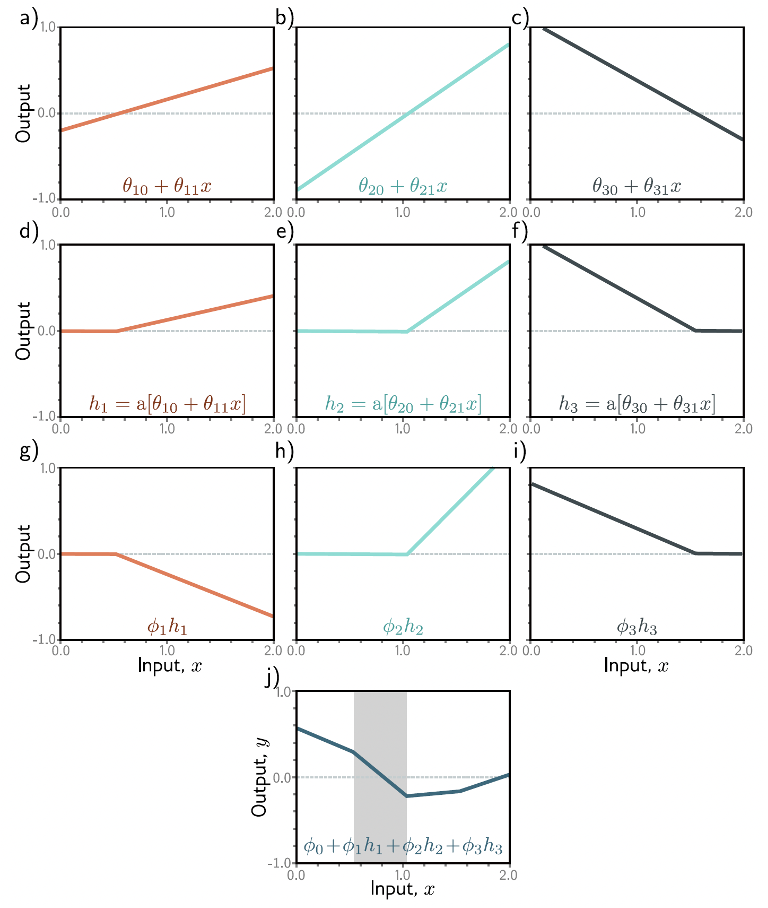
\includegraphics[width=0.5\textwidth]{shallow.png}
    \caption{Caption}
    \label{fig:shallow}
\end{figure}

\solutionspace{4cm}{15cm}{}{
Based on plots d-f in the figure:

Region 1 (leftmost, x < -θ₁₀/θ₁₁): All units inactive (h₁, h₂, h₃ all have zero output)
Region 2 (-θ₁₀/θ₁₁ < x < -θ₂₀/θ₂₁): Only h₁ active, h₂ and h₃ inactive
Region 3 (-θ₂₀/θ₂₁ < x < -θ₃₀/θ₃₁): h₁ and h₂ active, h₃ inactive
Region 4 (rightmost, x > -θ₃₀/θ₃₁): All units (h₁, h₂, h₃) active

The activation pattern can be confirmed by examining plots d-f, which show each ReLU unit becoming active at different threshold points.}

\end{question}

\begin{question}[8] Derive expressions for the positions of the "joints" in function in figure~\ref{fig:shallow}j
in terms of the ten parameters $\phi$ and the input $x$. 

\solutionspace{4cm}{15cm}{}{
The joints occur at the activation thresholds:

Joint 1: x = -θ₁₀/θ₁₁ (where h₁ activates)
Joint 2: x = -θ₂₀/θ₂₁ (where h₂ activates)
Joint 3: x = -θ₃₀/θ₃₁ (where h₃ activates)

These points represent where each ReLU activation begins.}

\end{question}

\begin{question}[8] Derive expressions for the slopes of the four
linear regions in figure~\ref{fig:shallow}j.


\solutionspace{4cm}{15cm}{}{
The slopes in each region are:

Region 1: 0 (no active units)
Region 2: φ₁θ₁₁ (only h₁ contributes)
Region 3: φ₁θ₁₁ + φ₂θ₂₁ (h₁ and h₂ contribute)
Region 4: φ₁θ₁₁ + φ₂θ₂₁ + φ₃θ₃₁ (all units contribute)

Each slope represents the cumulative effect of active units.}

\end{question}

\end{problem}

 
\begin{problem} {Deep neural networks}





\begin{question}[8] Consider composing the two neural networks shown in Figure~\ref{fig:deep}. Plot the relationship between the input \( x \) and the output \( y' \) for \( x \in [-1, 1] \).
\begin{figure}[htbp]
    \centering
    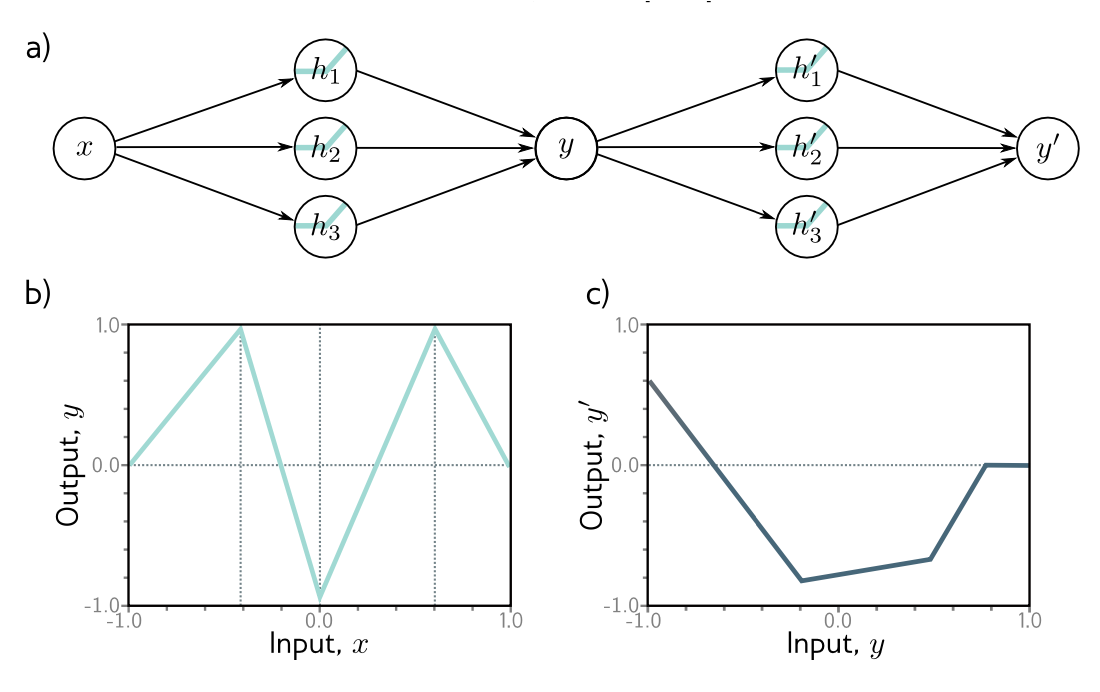
\includegraphics[width=0.6\textwidth]{deep.png}
    \caption{Composition of two networks. a) The output y of the
first network becomes the input to the second. b) The first network computes
this function with output values $y \in [-1,1]$. c) The second network computes this function on the input range $y \in [-1,1]$.}
    \label{fig:deep}
\end{figure}

    \solutionspace{4cm}{15cm}{}{
The composed network maps input x to output y' by:
1. First mapping x to y using network 1
2. Then mapping that y to y' using network 2

Following this composition point-by-point:

For x ∈ [-1, 0]:
- First network: y increases linearly from 0 to 1 (as shown in figure b)
- Second network: When y increases from 0 to 1, y' decreases linearly from 0 to -0.8 (as shown in figure c)

For x ∈ [0, 1]:
- First network: y decreases linearly from 1 to -1
- Second network: When y decreases from 1 to -1, y' increases from -0.8 to 0

The result is a V-shaped continuous piecewise linear function with minimum y' = -0.8 at x = 0.}
    
\end{question}

 
 \begin{question}[8] Identify the hyperparameters in figure~\ref{fig:deep2}. (Hint: there are four!)

\begin{figure}[htbp]
    \centering
    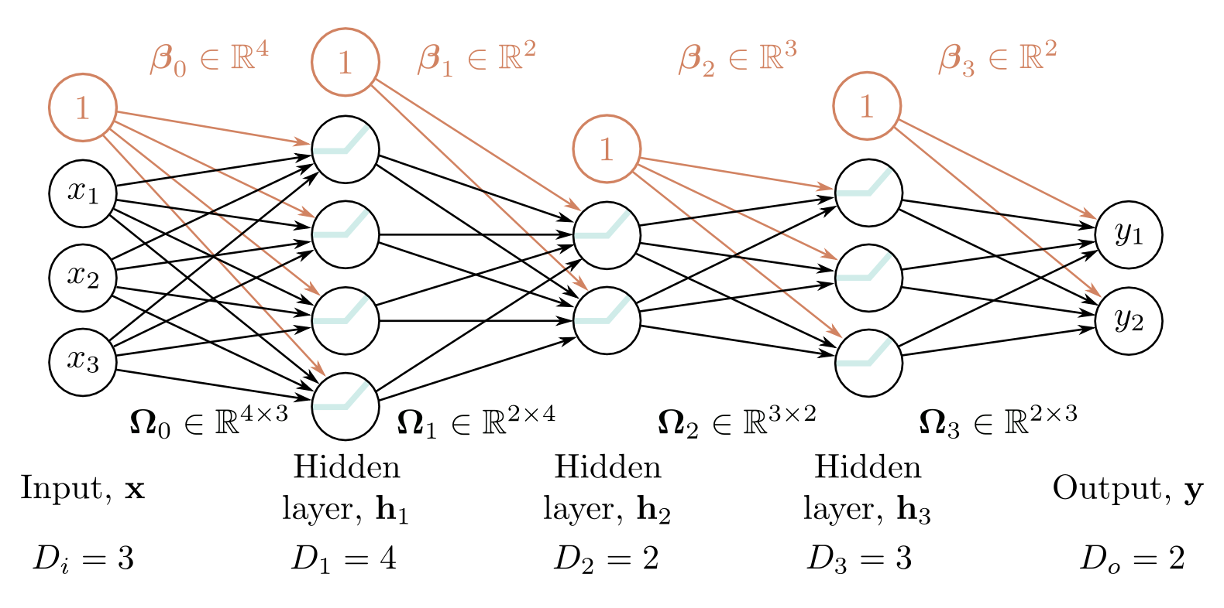
\includegraphics[width=0.6\textwidth]{deep2.png}
    \caption{Matrix notation for a network with \( D_i = 3 \)-dimensional input \( \mathbf{x} \), \( D_o = 2 \)-dimensional output \( \mathbf{y} \), and \( K = 3 \) hidden layers \( \mathbf{h}_1, \mathbf{h}_2, \mathbf{h}_3 \) of dimensions \( D_1 = 4 \), \( D_2 = 2 \), and \( D_3 = 3 \), respectively. The weights are stored in matrices $\Omega$
that multiply the activations from the preceding layer to create the pre-activations
at the subsequent layer.}
    \label{fig:deep2}
\end{figure}


  \solutionspace{4cm}{15cm}{}{
The four hyperparameters from the network diagram are:

1. Input dimension D_i = 3 (number of input features)
2. Output dimension D_o = 2 (number of outputs)
3. Number of hidden layers K = 3 (depth of network)
4. Hidden layer dimensions: D₁ = 4, D₂ = 2, D₃ = 3 (width of each layer)

These parameters fully specify the network architecture.}
  
\end{question}


 \begin{question}[8] the non-negative homogeneity property of the ReLU function indicates that  \[ \text{ReLU}(\alpha z) = \alpha \cdot \text{ReLU}(z) \]

Please show the following identity involving the ReLU function and non-negative scalars \( \lambda_0, \lambda_1 \geq 0 \): \[ \text{ReLU}\left[\beta_1 + \lambda_1 \cdot \Omega_1 \, \text{ReLU} \left[\beta_0 + \lambda_0 \cdot \Omega_0 x \right] \right] = \lambda_0 \lambda_1 \cdot \text{ReLU} \left[ \frac{1}{\lambda_0 \lambda_1} \beta_1 + \Omega_1 \, \text{ReLU} \left[ \frac{1}{\lambda_0} \beta_0 + \Omega_0 x \right] \right] \]
  \solutionspace{15cm}{15cm}{}{
Let's prove this step by step:

1. Start with left side: ReLU[β₁ + λ₁Ω₁ReLU[β₀ + λ₀Ω₀x]]

2. Using homogeneity on inner ReLU:
   = ReLU[β₁ + λ₁Ω₁(λ₀ReLU[1/λ₀(β₀ + λ₀Ω₀x)])]
   = ReLU[β₁ + λ₀λ₁Ω₁ReLU[1/λ₀β₀ + Ω₀x]]

3. Factor out λ₀λ₁:
   = ReLU[λ₀λ₁(1/(λ₀λ₁)β₁ + Ω₁ReLU[1/λ₀β₀ + Ω₀x])]

4. Apply homogeneity property again:
   = λ₀λ₁ReLU[1/(λ₀λ₁)β₁ + Ω₁ReLU[1/λ₀β₀ + Ω₀x]]

Which gives us the right side of the equation.}
  
\end{question}


\end{problem}


\begin{problem} {Loss Functions} 


 \begin{question} Suppose we want to build a neural network that predicts the wind direction \( y \), in radians, based on local measurements of barometric pressure \( x \). A suitable choice for modeling distributions over circular domains is the \textit{von Mises distribution}\footnote{\url{https://en.wikipedia.org/wiki/Von_Mises_distribution}}:

\begin{equation}
\Pr(y \mid \mu, \kappa) = \frac{\exp\left(\kappa \cos(y - \mu)\right)}{2\pi I_0(\kappa)},
\end{equation}

where \( \mu \) denotes the mean direction and \( \kappa > 0 \) is a concentration parameter, which plays a role analogous to the inverse of variance in a normal distribution. The term \( I_0(\kappa) \) represents the modified Bessel function of the first kind, of order 0.

The von Mises distribution is defined on the circular domain \( (-\pi, \pi] \). It is fully characterized by its two parameters: the mean \( \mu \), which controls the location of the peak, and the concentration \( \kappa \), which determines how tightly the distribution is clustered around the mean. Roughly speaking, \( 1/\sqrt{\kappa} \) corresponds to the standard deviation in the normal distribution.

\begin{subquestion}[8] Please develop a loss function for learning the parameter \( \mu \) of a model \( f[x, \boldsymbol{\phi}] \) that predicts the most likely wind direction. Assume the concentration parameter \( \kappa \) is constant.  

  \solutionspace{5cm}{15cm}{}{
For the von Mises distribution with fixed κ, the proper loss function is:

L = -κcos(y - μ)

Derivation:
1. Take negative log-likelihood of von Mises distribution:
   -log(Pr(y|μ,κ)) = -log[exp(κcos(y-μ))/(2πI₀(κ))]
   = -κcos(y-μ) + log(2πI₀(κ))

2. Since κ is constant, log(2πI₀(κ)) is constant and doesn't affect optimization
   L = -κcos(y-μ)

3. For optimization purposes, we can further simplify to:
   L = -cos(y-μ)

This loss correctly handles the circular nature of wind direction data where 
angles that differ by 2π are equivalent.}

\end{subquestion}

\begin{subquestion}[4] How would you perform inference?

  \solutionspace{5cm}{15cm}{}{
For inference with the trained model:

1. Forward pass: Input barometric pressure x through model f[x,φ] to get the predicted mean direction μ = f[x,φ]

2. Ensure prediction is in proper range: Since wind direction is circular, normalize μ to (-π,π] using:
   μ_normalized = ((μ + π) % 2π) - π

3. Return μ_normalized as the predicted most likely wind direction

4. The uncertainty of this prediction is determined by κ (higher κ means more confidence)
   - Standard deviation approximation: σ ≈ 1/√κ
   - 95% confidence interval: μ ± 2σ (adjusting for circular nature)

This approach correctly handles the periodicity of directional data.}
  
  \end{subquestion}
   
\end{question}


\begin{question}[8]
Construct a loss function for making multivariate predictions $y$ based on independent normal distributions with different variances $\sigma^2_d$
d for each dimension. Assume that this is a
heteroscedastic model so that both the means $\mu_d$ and variances $\sigma^2_d$ change as a function of the
data.

 \solutionspace{5cm}{15cm}{}{
For heteroscedastic multivariate normal predictions with D dimensions, the proper loss function is:

L = Σᵈᵢ₌₁ [(yᵢ - μᵢ(x))²/(2σᵢ²(x)) + (1/2)log(2πσᵢ²(x))]

Where:
- μᵢ(x) is the predicted mean for dimension i as a function of input x
- σᵢ²(x) is the predicted variance for dimension i as a function of input x
- yᵢ is the true value for dimension i

This is derived from the negative log-likelihood of a product of independent normal distributions:
p(y|x) = Πᵈᵢ₌₁ N(yᵢ|μᵢ(x),σᵢ²(x))

The model outputs 2D values: D means and D variances, allowing it to express both:
1. The expected value for each dimension (μᵢ)
2. The uncertainty of that prediction (σᵢ²)

This formulation naturally balances the desire for accurate predictions with appropriate 
uncertainty estimation. High variance predictions incur less penalty for errors but pay a "cost" 
through the log term, preventing the model from always predicting infinite variance.}
  
\end{question}


\begin{question}[12]
Consider a multivariate regression problem in which we predict the height of an individual in meters and their weight in kilos from some data x. Here, the units take quite different values. What problems do you see this causing? Propose two solutions to these problems.


 \solutionspace{5cm}{15cm}{}{
Problems:
1. Scale Disparity:
   - Height typically ranges 1.5-2.0 meters
   - Weight typically ranges 45-120 kilos
   - This ~60x difference in scales means weight errors will dominate the loss function

2. Training Issues:
   - Gradient updates will be imbalanced
   - Model will prioritize weight accuracy over height
   - Learning rate that works for weight may be too large/small for height
   - Risk of numerical instability in computations

Solutions:
1. Data Normalization:
   - Standardization: (x - μ)/σ for each feature
   - Makes both height and weight zero-mean, unit variance
   - Ensures equal scale influence on loss function
   - Can easily convert back to original units after prediction

2. Custom Loss Function:
   - Use weighted MSE: α₁(h_pred - h_true)² + α₂(w_pred - w_true)²
   - Set α₁, α₂ inversely proportional to typical squared ranges
   - Example: α₁ = 1, α₂ = (0.5)² to account for scale differences
   - Allows explicit control over importance of each prediction}
  
\end{question}

\end{problem}

\begin{problem} {Fitting models}

\begin{question}[10]
Please compute the derivatives of the least squares loss \( L[\boldsymbol{\phi}] \) with respect to the Gabor model parameters \( \boldsymbol{\phi} = (\phi_0, \phi_1) \) discussed in Lecture 20.

 \solutionspace{10cm}{15cm}{}{
For the Gabor model f(x) = φ₀ + φ₁cos(x), we first define the least squares loss:

L[φ] = (1/2)Σᵢ (f(xᵢ,φ) - yᵢ)² 
     = (1/2)Σᵢ (φ₀ + φ₁cos(xᵢ) - yᵢ)²

The derivatives with respect to each parameter are:

∂L/∂φ₀ = Σᵢ (φ₀ + φ₁cos(xᵢ) - yᵢ)
       = Σᵢ (f(xᵢ) - yᵢ)

∂L/∂φ₁ = Σᵢ (φ₀ + φ₁cos(xᵢ) - yᵢ)cos(xᵢ)
       = Σᵢ (f(xᵢ) - yᵢ)cos(xᵢ)

These gradients have an intuitive interpretation:
- ∂L/∂φ₀ is proportional to the total prediction error
- ∂L/∂φ₁ weights each error by cos(xᵢ), giving more importance to points 
  where the cosine feature has higher magnitude

Setting these derivatives to zero and solving would give the optimal parameters.}
 
\end{question}

\begin{question}[10]
Compute the gradients of the least squares loss with respect to the ten parameters of the simple neural network model presented in the 'Shallow Network' example from Lecture 18.

 \solutionspace{10cm}{15cm}{}{
For our shallow neural network with ReLU activations:
f(x) = φ₀ + φ₁ReLU(θ₁₀ + θ₁₁x) + φ₂ReLU(θ₂₀ + θ₂₁x) + φ₃ReLU(θ₃₀ + θ₃₁x)

The least squares loss gradients for all ten parameters are:

1. Output weights and bias:
   ∂L/∂φ₀ = Σᵢ (f(xᵢ) - yᵢ)
   ∂L/∂φⱼ = Σᵢ (f(xᵢ) - yᵢ)ReLU(θⱼ₀ + θⱼ₁xᵢ)     for j ∈ {1,2,3}

2. Hidden layer parameters:
   ∂L/∂θⱼ₀ = Σᵢ (f(xᵢ) - yᵢ)φⱼ1[θⱼ₀ + θⱼ₁xᵢ > 0]  for j ∈ {1,2,3}
   ∂L/∂θⱼ₁ = Σᵢ (f(xᵢ) - yᵢ)φⱼxᵢ1[θⱼ₀ + θⱼ₁xᵢ > 0] for j ∈ {1,2,3}

Where:
- 1[condition] is the indicator function (equals 1 when condition is true, 0 otherwise)
- ReLU(z) = max(0,z)
- θⱼ₀ and θⱼ₁ are the bias and weight for hidden unit j
- φⱼ is the output weight for hidden unit j

Notice how the ReLU activation introduces a discontinuity in the gradients through 
the indicator function. This means neurons only receive gradient updates when they're 
active (θⱼ₀ + θⱼ₁xᵢ > 0), which is a defining characteristic of ReLU networks.}

\end{question}

\end{problem}


\end{document}
